\section{Method}
\label{sec:method}

\begin{figure}

		\centering
		
		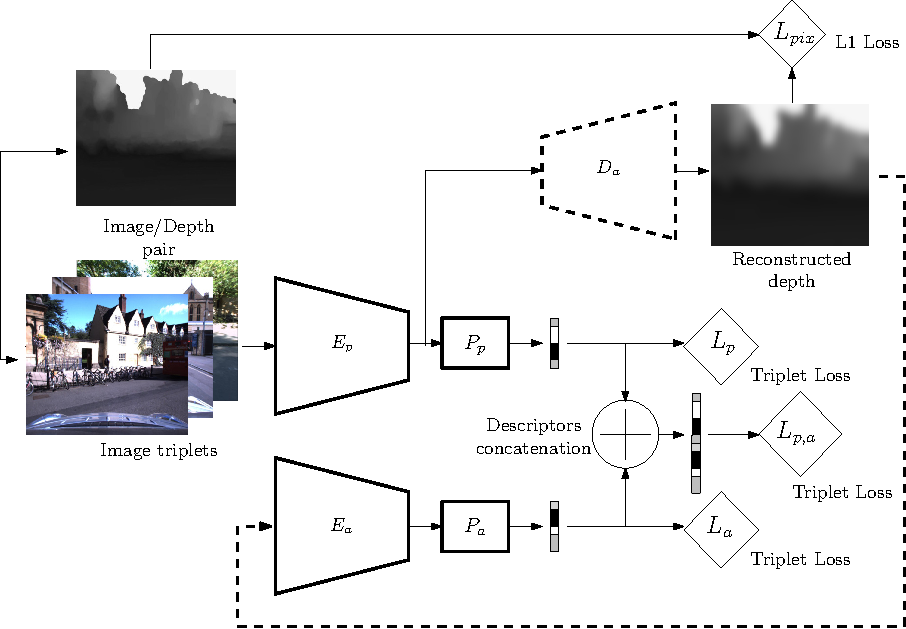
\includegraphics[width=\linewidth]{method/our_method_training}
		\caption[Image descriptors training with auxiliary depth data]{\label{fig:our_method} \textbf{Image descriptors training with auxiliary depth data (our work):} two encoders are used for extracting deep features map from the main image modality and the auxiliary reconstructed depth map (inferred from our deep decoder). These features are used to create intermediate descriptors that are finally concatenated in one final image descriptor.}	

\end{figure}
	
%\begin{figure}
	\center
	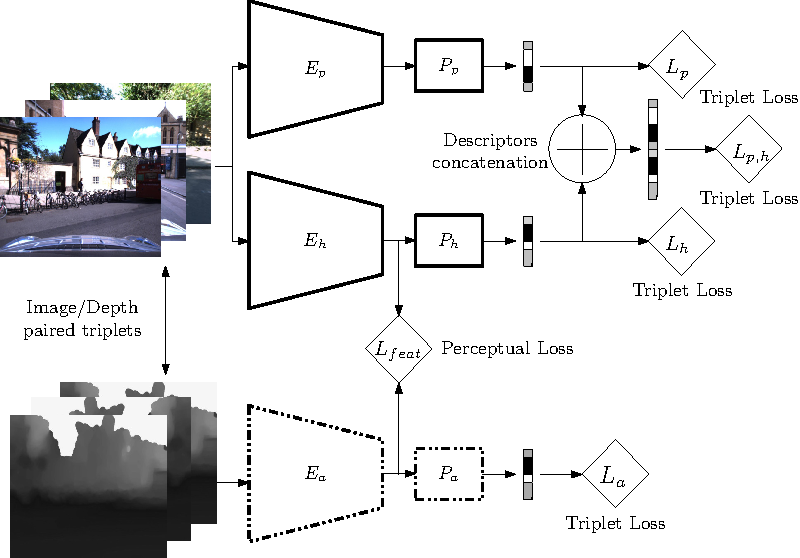
\includegraphics[width=\linewidth]{method/hall_method_training}
	\caption{\label{fig:hall_method} \textbf{Hallucination network for image descriptors learning:} we train an hallucination network, inspired from~\cite{Hoffman2016}, for the task of global image description. Unlike the proposed method (see figure~\ref{fig:our_method}), hallucination network reproduces feature maps that would have been obtained by a network trained with depth map rather than the deep map itself.}
\end{figure}


We use the same descriptor architecture introduced in~\cite{Piasco2019}. The method, presented in figure~\ref{fig:our_method}, is composed of:

\begin{itemize}
	\item a CNN image encoder $E_I$ linked to a features aggregation layer $d_I$ that produce a compact image descriptor,
	\item a CNN image decoder $D_G$ used to reconstruct the corresponding depth map according to the monocular image,
	\item a CNN depth map encoder $E_D$ linked to a features aggregation layer $d_D$ that produce a compact depth map descriptor,
	\item a fusion module that concatenate the image and depth map descriptor.
\end{itemize}

\subsection{Training routine}
\label{subsec:training}
Trainable parameters are $\theta_{I}$ the weights of encoder and descriptor $\{E_I, d_I\}$, $\theta_{D}$ the weights of the encoder and descriptor $\{E_D, d_D\}$ and $\theta_{G}$ the weights of the decoder used for depth map generation. 

For training our system, we follow standard procedure of descriptor learning based on triplet margin losses~\cite{Arandjelovic2017}. A triplet $\{q_{im}, q_{im}^+, q_{im}^-\}$ is composed of an anchor image $q_{im}$, a positive example $q_{im}^+$ representing the same scene as the anchor and an unrelated negative example $q_{im}^-$.
The first triplet loss acting on $\{E_I, d_I\}$ is:
\begin{equation}
	\label{eq:triplet_loss}
	L_{f_{\theta_{I}}}(q_{im}, q_{im}^+, q_{im}^-) = max\left(\lambda + \norm{f_{\theta_{I}}(q_{im}) - f_{\theta_{I}}(q_{im}^+)}_2 - \norm{f_{\theta_{I}}(q_{im}) - f_{\theta_{I}}(q_{im}^-)}_2, 0 \right),
\end{equation}
where $f_{\theta_{I}}(x_{im})$ is the global descriptor of image $x_{im}$ and $\lambda$ an hyper-parameter controlling the margin between positive and negative examples. $f_{\theta_{I}}$ can be written as:
\begin{equation}
	\label{eq:desc_details}
	f_{\theta_{I}}(x_{im}) = d_I(E_I(x_{im})),
\end{equation}
where $E_I(x_{im})$ represents the deep feature maps extracted by the decoder and $d_I$ the function used to build the final descriptor from the feature.

We train the depth map encoder and descriptor $\{E_D, d_D\}$ in a same manner, with the triplet loss of equation~(\ref{eq:triplet_loss}), $L_{f_{\theta_{D}}}(\hat{q}_{depth}, \hat{q}_{depth}^+, \hat{q}_{depth}^-)$, where $f_{\theta_{D}}(x_{depth})$ is the global descriptor of depth map $x_{depth}$ and $\hat{x}_{depth}$ is the reconstructed depth map of image $x_{im}$ by the decoder $D_G$:
\begin{equation}
	\label{eq:generator}
	\hat{x}_{depth} = D_G(E_I(x_{im})).
\end{equation}
Decoder $D_G$ uses the deep representation of image $x_{im}$ computed by encoder $E_I$ in order to reconstruct the scene geometry. Notice that even if the encoder $E_I$ is not especially trained for depth map reconstruction, its intern representation is rich enough to be used by the decoder $D_G$ for the task of depth map inference. We choose to use the features already computed by the first encoder $E_I$ instead of introducing another encoder for saving computational resources.

The final image descriptor is trained with the triplet loss $L_{F_{\theta_{I}, \theta_{D}}}({q}_{im}, {q}_{im}^+, {q}_{im}^-)$, where $F_{\theta_{I},\theta_{D}}(x_{im})$ denotes the fusion of image descriptor and depth map descriptor: 
\begin{equation}
	\label{eq:desc_fuse}
	F_{\theta_{I},\theta_{D}}(x_{im}) = fuse \left( f_{\theta_{I}}(x_{im}), f_{\theta_{D}}(\hat{x}_{depth}) \right).
\end{equation}

In order to train the depth map generator, we use a simple $L_1$ loss function:
\begin{equation}
 \label{eq:l1_loss}
	L_{\theta_{G}} = \norm{x_{depth} - \hat{x}_{depth}}_{1}.
\end{equation}

The whole system is trained according to the following constraints:
\begin{align}
	\left( \theta_{I}, \theta_{D} \right) & := arg\,\underset{\theta_{I}, \theta_{D}}{min} \left[ L_{f_{\theta_{I}}} + L_{f_{\theta_{D}}} + L_{F_{\theta_{I},\theta_{D}}} \right], \label{eq:sys_optimization_1} \\ 	
	\left( \theta_{G} \right) & := arg\,\underset{\theta_{G}}{min} \left[ L_{\theta_{G}} \right]. 	\label{eq:sys_optimization_2}
\end{align}

We use two different optimizers: one updating $\theta_{I}$ and $\theta_{D}$ weights regarding constraint~(\ref{eq:sys_optimization_1}) and the other updating $\theta_{G}$ weights regarding constraint~(\ref{eq:sys_optimization_2}). Because decoder $D_G$ relies on feature maps computed by encoder $E_I$ (see equation~(\ref{eq:generator})), at each optimization step on $\theta_{I}$ we need to update decoder weights $\theta_{G}$ to take in account possible changes in the image features. We finally train our entire system, by alternating between the optimization of weights $\{\theta_{I}, \theta_{D}\}$ and $\{\theta_G\}$ until convergence.

\subsection{Hard mining}


\subsection{Descriptors fusion and dimension reduction}
\label{subsec:fuse_desc}
We test several descriptors fusion function, the one introduced in equation~\ref{eq:desc_fuse}, in order to benefit as much as possible of the complementarity of the main and the auxiliary modalities. We compare: simple descriptors concatenation, hand-tuned descriptors scalar weighting, trained scalar weighting~\cite{Sizikova2016}, trained modal attention mechanism at the level of descriptors and trained spatial and modal attention mechanism at the level of deep features~\cite{Seymour2018}. We found that all the fusion policies perform equally, so we use the simple concatenation operator to fuse the descriptors. Actually, the modalities fusion is learned by our system through the triplet loss $L_{F_{\theta_{I}, \theta_{D}}}$, making the system aware of what is important and complementary in the radiometric and geometric domain without the need of complex fusion methods.

We can reduce the dimension of the final descriptor by applying PCA + whitening~\cite{Arandjelovic2017, Radenovic2017, Gordo2017}. After the convergence of the whole system we reuse the images from the training dataset to compute the PCA parameters.

\subsection{Side information learning with hallucination}
\label{subsec:hall}

knowledge distillation~\citep{hinton2015distilling}

We compare our method of side information learning with a state-of-the-art approach system, named hallucination network~\cite{Hoffman2016}. The hallucination network is originally designed for object detection and classification in images. We adapt the work of~\cite{Hoffman2016} to create an image descriptor system that benefits from depth map side modality during training. Like our proposal, the trained hallucination network is used on images only and produce a global descriptor for image localization. The system is presented in figure~\ref{fig:hall_method}. The main difference with our proposal is that the hallucination network reproduces feature maps that would have been obtained by a network trained with depth map rather than the deep map itself. We refer readers to~\cite{Hoffman2016} for more information about the hallucination network.

\vspace{4pt}\noindent\textit{Advantages and drawbacks.}
\label{paragraph:adv}
One advantage of the hallucination network over our proposal is that it does not require a decoder network, resulting on a architecture lighter than ours. However, it needs a pre-training step, where image encoder and depth map encoder are trained separately from each other before a final optimization step with the hallucination part of the system. Our system do not need such initialization. Training the hallucination network requires more complex data than the proposed method. Indeed, it needs to gather triplets of image, and depth map pairs, which require to know the absolute position of the data~\cite{Arandjelovic2017,Liu2018}, or to use costly algorithms like Structure from Motion (SfM)~\cite{Godard2017,Radenovic2017,Kim2017a}. 

One advantage of our method over the hallucination approach is that we have two unrelated objectives during training: learning a efficient image representation for localization and learning how to reconstruct scene geometry from an image. It means we can train several parts of our system separately, with different source of data. Especially, we can improve the scene geometry reconstruction task with non localized \textit{\{image, depth map\}} pairs. These weakly annotated data are easier to gather than triplet, as we only need calibrated system capable of sensing radiometric and geometric modalities at the same time. We will show in practice how this can be exploited to fine tune the decoder part to deal with complex localization scenarios in part~\ref{subsec:results}.
